\section{eo\-Ctrl\-CContinue$<$ EOT $>$ Class Template Reference}
\label{classeo_ctrl_c_continue}\index{eoCtrlCContinue@{eoCtrlCContinue}}
Ctrl C handling: this {\bf eo\-Continue}{\rm (p.\,\pageref{classeo_continue})} tells whether the user pressed Ctrl C.  


{\tt \#include $<$eo\-Ctrl\-CContinue.h$>$}

Inheritance diagram for eo\-Ctrl\-CContinue$<$ EOT $>$::\begin{figure}[H]
\begin{center}
\leavevmode
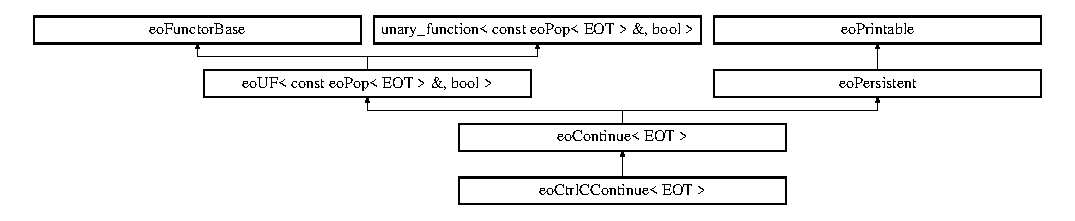
\includegraphics[height=2.52252cm]{classeo_ctrl_c_continue}
\end{center}
\end{figure}
\subsection*{Public Member Functions}
\begin{CompactItemize}
\item 
{\bf eo\-Ctrl\-CContinue} ()\label{classeo_ctrl_c_continue_a0}

\begin{CompactList}\small\item\em Ctor : installs the signal handler. \item\end{CompactList}\item 
virtual bool {\bf operator()} (const {\bf eo\-Pop}$<$ {\bf EOT} $>$ \&\_\-v\-EO)\label{classeo_ctrl_c_continue_a1}

\begin{CompactList}\small\item\em Returns false when Ctrl C has been typed in reached. \item\end{CompactList}\item 
virtual std::string {\bf class\-Name} (void) const \label{classeo_ctrl_c_continue_a2}

\end{CompactItemize}


\subsection{Detailed Description}
\subsubsection*{template$<$class EOT$>$ class eo\-Ctrl\-CContinue$<$ EOT $>$}

Ctrl C handling: this {\bf eo\-Continue}{\rm (p.\,\pageref{classeo_continue})} tells whether the user pressed Ctrl C. 



Definition at line 45 of file eo\-Ctrl\-CContinue.h.

The documentation for this class was generated from the following file:\begin{CompactItemize}
\item 
eo\-Ctrl\-CContinue.h\end{CompactItemize}
